\documentclass[12pt]{article}
\usepackage{amsmath}
\usepackage{booktabs}
\usepackage{graphicx}

\title{Discrete Assignment-11.9.1-11}
\author{Hiba Muhammed \\
        EE23BTECH11026}
\date{} % Remove the date since it's auto-generated

\begin{document}

\maketitle

\section*{Problem Statement}
Write the first five terms in the sequence:
\begin{align*}
a_{0}  &= 3 \\
a_{n}  &= 3a_{n-1} + 2 \quad \text{for } n > 0
\end{align*}

\section*{Solution}
\begin{table}[h]
  \centering
  \caption{Input Parameters: First Term and General Formula}
  \begin{tabular}{|c|c|}
    \hline
    \textbf{Term} & \textbf{Value} \\
    \hline
    \(x(0)\) & 3 \\
    \(x(n)\) & \(3x(n-1) + 2\) \\
    \hline
  \end{tabular}
\end{table}

Let's find the first 5 terms of the sequence:
\begin{align*}
x(1) &= 3x(0) + 2 = 3 \times 3 + 2 = 11 \\
x(2) &= 3x(1) + 2 = 3 \times 11 + 2 = 35 \\
x(3) &= 3x(2) + 2 = 3 \times 35 + 2 = 107 \\
x(4) &= 3x(3) + 2 = 3 \times 107 + 2 = 323 \\
x(5) &= 3x(4) + 2 = 3 \times 323 + 2 = 971 
\end{align*}

So, the first 5 terms of the sequence are \(3, 11, 35, 107, 323\).

Consider the difference equation \(x(n) = 3x(n-1) + 2u(n)\). The Z-transform of this difference equation is
\begin{align*}
X(z) &= \frac{2}{(1 - z^{-1})(1 - 3z^{-1})} \\
&= \frac{A_1}{1 - z^{-1}} + \frac{A_2}{1 - 3z^{-1}}
\end{align*}

To find the values of \(A_1\) and \(A_2\), multiply through by the common denominator:
\begin{equation}
1 = A_1(1-3z^{-1}) + A_2(1-z^{-1})
\end{equation}

Equating coefficients, solve for \(A_1\) and \(A_2\):
\begin{align*}
A_1 &= -1 \\
A_2 &= 3
\end{align*}

Substitute these values back into the modified partial fraction decomposition:
\begin{align*}
X(z) &= -\frac{1}{1-z^{-1}} + \frac{3}{1-3z^{-1}} \\
\end{align*}

Now, find the inverse \(Z\)-transform of each term using the property \(Z^{-1}\left[\frac{1}{1-cz^{-1}}\right] = c^n u_n\). The result is:
\begin{equation}
x_n = -u_n + 3(3^n u_n)
\end{equation}

\begin{figure}[h]
    \centering
    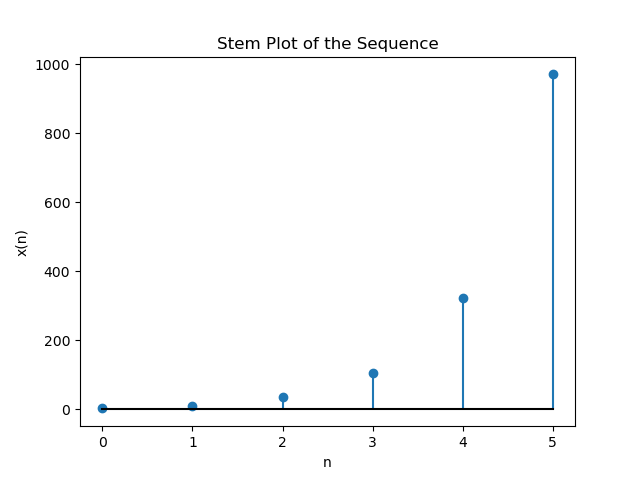
\includegraphics[width=0.7\linewidth]{11.9.1-11.png}
    \caption{Sequence plot generated from the Python script.}
    \label{fig:sequence-plot}
\end{figure}

\begin{figure}[h]
  \centering
  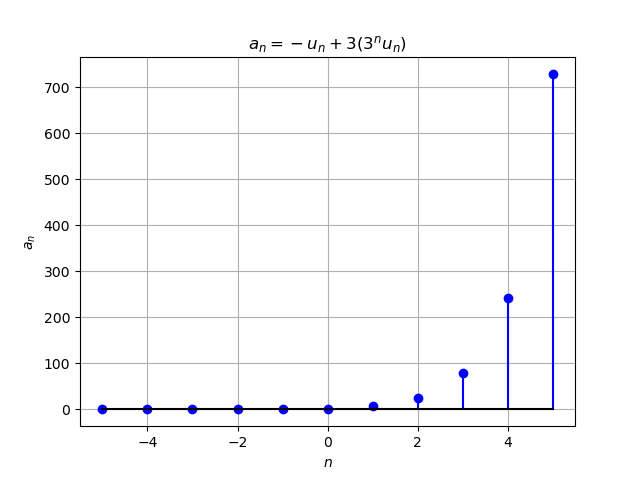
\includegraphics[width=0.8\linewidth]{11.9.1-11x.png} % Replace with the path to your saved image file
  \caption{Plot of the sequence \(a_n = -u_n + 3(3^n u_n)\)}
  \label{fig:sequence_plot}
\end{figure}

\end{document}

